\documentclass[12pt, oneside]{article}   	% use "amsart" instead of "article" for AMSLaTeX format

\usepackage{graphicx}
\graphicspath{ {\string} }
\usepackage{subcaption}

%%%%%%%%%%%%%%%%%%%%%%%%%%%%%%%%%%%%%%%%%%%%%%%%%%%%
% set up packages
%%%%%%%%%%%%%%%%%%%%%%%%%%%%%%%%%%%%%%%%%%%%%%%%%%%%
\usepackage{geometry}                
\usepackage{textcomp}                
\usepackage{amsmath}                
\usepackage{graphicx}                
\usepackage{amssymb}                
\usepackage{fancyhdr}                
\usepackage{subcaption}                
\usepackage{bm}                
\usepackage{lineno}
% package for comments
\usepackage{soul}     
\usepackage{setspace}

%%%%%%%%%%%%%%%%%%%%%%%%%%%%%%%%%%%%%%%%%%%%%%%%%%%%
% call packages
%%%%%%%%%%%%%%%%%%%%%%%%%%%%%%%%%%%%%%%%%%%%%%%%%%%%	
\geometry{letterpaper, marginparwidth=60pt} % sets up geometry              		
\linenumbers % adds line numbers 
\doublespacing % setspace
	
\usepackage[superscript,noadjust]{cite} % puts dash in citations to abbreviate
%\usepackage [autostyle, english = american]{csquotes} % sets US-style quotes
%\MakeOuterQuote{"} % sets quote style

\usepackage{hyperref}
\hypersetup{
    colorlinks=true,
    linkcolor=blue,
    filecolor=magenta,      
    urlcolor=cyan,
}

\usepackage{tabularx}

\usepackage{etoolbox}
\AtBeginEnvironment{quote}{\small}

\usepackage{float,color}
\usepackage{xcolor}
\definecolor{darkspringgreen}{rgb}{0.09, 0.45, 0.27}

\usepackage[section]{placeins}

\usepackage{tikz-qtree}
\usetikzlibrary{trees}

\usepackage{natbib}
%\bibliographystyle{abbrvnat}
\setcitestyle{authoryear,open={(},close={)}}

%%%%%%%%%%%%%%%%%%%%%%%%%%%%%%%%%%%%%%%%%%%%%%%%%%%%

%%%%%%%%%%%%%%%%%%%%%%%%%%%%%%%%%%%%%%%%%%%%%%%%%%%%
\pagestyle{plain}                                                      %%
%%%%%%%%%% EXAFT 1in MARGINS %%%%%%%                                   %%
\setlength{\textwidth}{6.5in}     %%                                   %%
\setlength{\oddsidemargin}{0in}   %% (It is recommended that you       %%
\setlength{\evensidemargin}{0in}  %%  not change these parameters,     %%
\setlength{\textheight}{8.5in}    %%  at the risk of having your       %%
\setlength{\topmargin}{0in}       %%  proposal dismissed on the basis  %%
\setlength{\headheight}{0in}      %%  of incorrect formatting!!!)      %%
\setlength{\headsep}{0in}         %%                                   %%
\setlength{\footskip}{.5in}       %%                                   %%
%%%%%%%%%%%%%%%%%%%%%%%%%%%%%%%%%%%%                                   %%		

%%%%%%%%%%%%%
% DEFINE CODE BLOCK
%%%%%%%%%%%%%
\usepackage{listings}

\definecolor{dkgreen}{rgb}{0,0.6,0}
\definecolor{gray}{rgb}{0.5,0.5,0.5}
\definecolor{mauve}{rgb}{0.58,0,0.82}

\lstset{frame=tb,
  language=R,
  aboveskip=3mm,
  belowskip=3mm,
  showstringspaces=false,
  columns=flexible,
  basicstyle={\small\ttfamily},
  numbers=none,
  numberstyle=\tiny\color{gray},
 % keywordstyle=\color{blue},
  commentstyle=\color{dkgreen},
  stringstyle=\color{mauve},
  breaklines=true,
  breakatwhitespace=true,
  tabsize=3,
  otherkeywords={0,1,2,3,4,5,6,7,8,9},
  deletekeywords={data,frame,length,as,character,dunif,ps},
}

%%%%%%%%%%%%%%%%%%%%%%%%%%%%%%%%%%%%%%%%%%%%%%%%%%%%
\usepackage{tikz}
\usetikzlibrary{arrows,automata}

%%%%%%%%%%%%%%%%%%%%%%%%%%%%%%%%%%%%%%%%%%%%%%%%%%%%

\usepackage{todonotes}

\begin{document} 

Prusinkiewicz et al. 2007 address the question of how inflorescence architecture is related to environmental variation. They look at how the fitness of different strategies varies across morphospace. Basically, they generate a fitness landscape for different parameter combinations. The authors then compare the fitness of different strategies. 

Following Neubert 2003, this seems to be different from identifying a strategy/the strategies that maximize fitness over all feasible strategies. (Or maybe it is similar?) The distinction is that there is [paraphrasing Neubert] no guarantee that the strategies considered maximize fitness over all feasible strategies. 

So I think the goal would be to come up with a set of possible decisions that could generate all possible architectures, and then optimize across all those possible strategies. 

I think this would be more difficult than what I had been trying to do before because it would involve (1) decisions about vegetative branching, (2) decisions about allocation to flowering, and (3) decisions about inflorescence branching. 

I wonder if it's possible to reduce the number of terms in any way?

\subsection*{Processes}

The model in Prusinkiewicz et al. 2007 does not include the effects of vegetative architecture. Studies on the genetic basis of vegetative and inflorescence branching suggest these are connected to differing degrees in different taxa. A review by Kellogg (2007?) of inflorescence branching in grasses suggest there is little relationship between the two. However, simplification of vegetative architecture in the domestication of teosinte to maize indicates there may be a relationship. 

I tried to consider the following. 
%
\begin{itemize}
  \item I assumed that plants must decide whether to allocate to `pure' vegetative development or transition to flowering. The probability that they undergo vegetative growth is $p(t)$ and the probability that they transition to flowering is $1-p(t)$. 
  \item I assumed that plants undergoing vegetative growth would have to decide whether to branch or not. Branching is the product of a decision about whether or not to produce a branch at an axillary position, or whether that position remains quiescent. The probability that a plant produces an axillary meristem is $x(t)$ and the probability that it does not, with the axillary position remaining quiescent, is $ 1 - x(t) $.
    \item Plants transition to flowering with probability $1-p(t)$. Plants that transition to flowering decide whether or not to completely transition to flowering along an axis. They might produce an inflorescence meristem, which terminates vegetative growth along the axis. Alternatively, they might produce a flower in an axillary position and permit continued vegetative growth along the main axis. The probability that a plant that has initiated flowering produces an inflorescence is $ y(t)$, and the probability that the plant produces an axillary floral meristem and continues vegetative growth along the main axis is $ 1 - y(t) $. Note that the value of this control is irrelevant if plants are not allocating to reproduction (i.e. if $p(t) = 1$) because the product of 0 and any value is 0. However, once flowering starts the decision becomes relevant. If plants produce an inflorescence meristem they are losing access to continued vegetative growth but ensuring continued commitment to flowering. If plants continue vegetative growth they immediately produce a flower and retain access to continued vegetative growth. They can also continue to divide by producing axillary meristems. However because axillary meristems were not produced the benefits do not accrue in the same way as if the plant had produced an axillary inflorescence with continued divisions producing more flowers on the branch as well as the main shoot. Note that these options do not permit for higher than second-order inflorescences but should hopefully allow us to investigate the question at hand irregardless.
    \item An inflorescence might be determinate, converting the branch into a terminal flower, or indeterminate, with continued growth along the inflorescence axis. The probability that an inflorescence terminates is $z(t)$ and the probability that it continues growth is $1-z(t)$. This formulation does not correspond to how determinate and indeterminate are used in the developmental biology literature: the former means that the main branch terminates in a flower while the later means it does not. However, both determinate and indeterminate plants can exhibit continuous growth along an axis, either from apical or axillary positions. For example, sympodial and monopodial growth can both be continuous and have similar life history consequences. I make the distinction that I'm not asking about architecture but rather about developmental decisions/meristem decisions. So the fitness consequences of racemose and cymose inflorescences are similar. 
\end{itemize}

Inflorescences can be determinate or indeterminate; terminating in a flower or continuing growth along an axis. They can also be simple (flowers on the main stem) or compound (flowers on branches). (Zhu and Wagner 2020; Coen and Nugent 1994). We focus on this and ignore whether an inflorescence is racemose/cymose, or bracteose/bractless (Coen and Nugent 1994).

During reproductive development, the inflorescence architecture can be determinate (i.e., terminate in a flower) or indeterminate; simple (flowers are borne on the main stem) or compound (flowers born on branches).

With that in mind, here are some of the decision patterns that might lead to particular architectures:

\begin{itemize}
  \item \textbf{Rosette with a single flower}. No vegetative branching ($x(t) = 0$); only a rosette is produced. Transition to flowering initiates an inflorescence ($y(t) = 1$). The inflorescence immediately terminates in a flower ($z(t) = 1$). [simple, determinate]
   \item \textbf{Rosette with a single inflorescence (this could be a raceme or a cyme)}. No vegetative branching ($x(t) = 0$); only a rosette is produced. Transition to flowering initiates an inflorescence ($y(t) = 1$). The inflorescence produces an inflorescence with axillary flowers ($z(t) = 0$). [simple, indeterminate]
    \item \textbf{Rosette with a single panicle}. No vegetative branching ($x(t) = 0$); only a rosette is produced initially. After a period of no branching, there is a brief period of branching ($x(t) = 1$). Transition to flowering on all branches initiates an inflorescence ($y(t) = 1$). The inflorescences immediately terminate in a flower ($z(t) = 1$). [compound, determinate]
    \item \textbf{Rosettes with a compound raceme }. No vegetative branching ($x(t) = 0$); only a rosette is produced. Transition to flowering on axillary branches initiates inflorescences on secondary branches ($y(t) = 0$). The inflorescence produces an inflorescence with axillary flowers ($z(t) = 0$). [compound, indeterminate]
  
\end{itemize}

I'm baffled by how to generate a panicle architecture (see Rao et al. 2007). For a panicle, there's a transition to flowering. The inflorescence meristem then generates primary branch meristems before terminating. The primary branch meristems generate secondary branch meristems before terminating in a spikelet. The secondary branch meristems also terminate in a spikelet. 

The discussion by Rao et al. 2007 suggests that maybe lateral branches in the panicle also retain transient expression of genes also involved in regulating axillary meristem growth. So maybe I can keep the processes in Figure 1 below and have them correspond to generate both vegetative and reproductive architecture. For example, a plant might initially not branch (1b) and then have a period of branching (1a) before reproduction. The decision to initiate flowering would then be (2a) followed by (3a). This creates a branched inflorescence with determinate terminals. 

(2b) should probably be option of transitioning to a inflorescence + floral meristem. This would be the equivalent of initiating a cyme (terminating the main axis in a flower and then adding flowers laterally. Or maybe this is no different than initiating a raceme? I need to read more on the development of these. 

Other things I'm not sure how to deal with: the distinction between racemes and cymes, panicle architecture, how to address determinate/indeterminate, simple/compound, etc. as part of this study. What's important?

\newpage

% vegetative development
\begin{figure}[hbt!]
  \begin{subfigure}[h]{.45\textwidth}
    \centering
    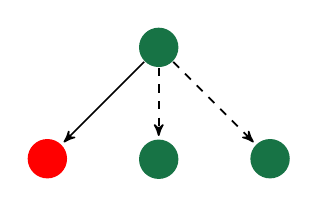
\begin{tikzpicture}[->,>=stealth',shorten >=1pt,auto,node distance=2cm,
                    semithick]
  \tikzstyle{every state}=[draw=none]

  \node[state, fill=darkspringgreen,minimum size=.5cm] 	     (A)                    {};
  \node[state, fill=red,minimum size=.5cm]         (B) [below left of=A] {};
  \node[state, fill=darkspringgreen,minimum size=.5cm]         (C) [below right of=A] {};
  \node[state, fill=darkspringgreen,minimum size=.5cm] 	     (D) [below =.9cm of A]                   {};

  \path[dashed] (A) edge              (D)
            	edge               (C);
  \path[->] (A) edge (B);

      \end{tikzpicture}
          \caption{Primary meristem transitioning to one vegetative meristem and generating two primary meristems. This process generates a main axis, axillary branch, and a leaf subtending the axillary branch.} 
  \end{subfigure}\
                \hspace{\fill}
   \begin{subfigure}[h]{.45\textwidth}
    \centering
    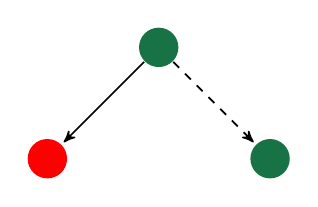
\begin{tikzpicture}[->,>=stealth',shorten >=1pt,auto,node distance=2cm,
                    semithick]
  \tikzstyle{every state}=[draw=none]

  \node[state, fill=darkspringgreen,minimum size=.5cm] 	     (A)                    {};
  \node[state, fill=red,minimum size=.5cm]         (B) [below left of=A] {};
  \node[state, fill=darkspringgreen,minimum size=.5cm]         (C) [below right of=A] {};

  \path[dashed] (A) edge              (C);
  \path[->] (A) edge (B);

      \end{tikzpicture}
          \caption{Primary meristem transitioning to one vegetative meristem and generating one primary meristems. This process generates a main axis and a leaf. } 
  \end{subfigure}\
        \caption{Meristem transitions for primary meristems subject to decisions about whether or not to branch.}
        \label{fig:transitions-1}
\end{figure}

% transition to flowering
\begin{figure}[hbt!]
  \begin{subfigure}[h]{.45\textwidth}
    \centering
    \centering

      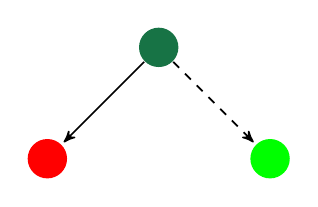
\begin{tikzpicture}[->,>=stealth',shorten >=1pt,auto,node distance=2cm,
                    semithick]
  \tikzstyle{every state}=[draw=none]

  \node[state, fill=darkspringgreen,minimum size=.5cm] 	     (A)                    {};
  \node[state, fill=red, minimum size=.5cm]         (B) [below left of=A] {};
  \node[state, fill=green, minimum size=.5cm]         (C) [below right of=A] {};

  \path[dashed] (A) edge              (C);
  \path[->] (A) edge (B);

      \end{tikzpicture}
          \caption{Primary meristem transitioning to one vegetative meristem and generating inflorescence meristems. This process initiates flowering along this axis.} 
  \end{subfigure} 
            \hspace{\fill}
  \begin{subfigure}[h]{.45\textwidth}
    \centering
    \centering

      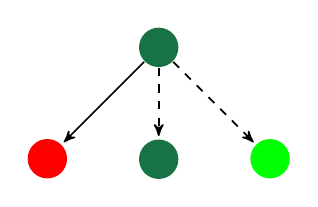
\begin{tikzpicture}[->,>=stealth',shorten >=1pt,auto,node distance=2cm,
                    semithick]
  \tikzstyle{every state}=[draw=none]

  \node[state, fill=darkspringgreen,minimum size=.5cm] 	     (A)                    {};
  \node[state, fill=red, minimum size=.5cm]         (B) [below left of=A] {};
    \node[state, fill=darkspringgreen, minimum size=.5cm]         (C) [below=.9cm of A] {};
  \node[state, fill=green, minimum size=.5cm]         (D) [below right of=A] {};

  \path[dashed] (A) edge              (C)
   			(A) edge              (D);
  \path[->] (A) edge (B);

      \end{tikzpicture}
          \caption{Primary meristem transitioning to one vegetative meristem and generating a floral and vegetative meristem.} 
  \end{subfigure} 
        \caption{Meristem transitions for primary meristems subject to decisions about flowering.}
        \label{fig:transitions-2}
\end{figure}

% inflorescence development
\begin{figure}[hbt!]   
  \begin{subfigure}[h]{.45\textwidth}
    \centering
    \centering

      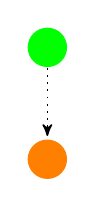
\begin{tikzpicture}[->,>=stealth',shorten >=1pt,auto,node distance=2cm,
                    semithick]
  %\tikzstyle{every state}=[fill=red,draw=none,text=white]

  \node[state, fill = green, draw = none,minimum size=.5cm] (A)                    {};
  \node[state, fill = orange, draw = none,minimum size=.5cm]         (B) [below=.9cm of A] {};

  \path[dotted] (A) edge              (B);

      \end{tikzpicture}
    \caption{Inflorescence meristem generating a floral meristem. This process generates a flower and terminates the axis.}
  \end{subfigure}\
            \hspace{\fill}  
  \begin{subfigure}[h]{.45\textwidth}
    \centering
    \centering

      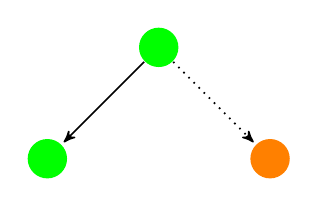
\begin{tikzpicture}[->,>=stealth',shorten >=1pt,auto,node distance=2cm,
                    semithick]
  %\tikzstyle{every state}=[fill=red,draw=none,text=white]

  \node[state, fill = green, draw = none,minimum size=.5cm] (A)                    {};
  \node[state, fill = green, draw = none,minimum size=.5cm]         (B) [below left of=A] {};
  \node[state, fill = orange, draw = none,minimum size=.5cm]         (C) [below right of=A] {};

  \path[dotted] (A) edge              (C);
  \path (A) edge		     (B);

      \end{tikzpicture}
    \caption{Inflorescence meristem remaining an inflorescence meristem and generating a floral meristem. This process generates a raceme, with flowers in axillary positions.}
  \end{subfigure}\
        \caption{Meristem transitions for inflorescence meristems subject to decisions about whether or not to branch.}
        \label{fig:transitions-3}
\end{figure}

\newpage


\subsection*{Description of diagram}

\subsubsection*{Vegetative growth: branching decisions}

The division shown in Figure \ref{fig:transitions-1}A occurs at a rate $\beta_1 p(t) x(t)$. The rate is the product of the ... ($\beta_1$), the probability with which primary meristems divide vegetatively ($p(t)$), and the probability with which primary meristem divisions generate axillary branching ($x(t)$). It results in the net gain of one primary meristem and gain of one vegetative meristem. The differential equations corresponding to this are:
%
\begin{align}
\dot{P} & = 2 \beta_1 p(t)  P - \beta_1 p(t) P = \beta_1 p(t) P \nonumber \\
\dot{V} & = \beta_1 p(t)  P      \nonumber \\
\dot{I} & = 0  \nonumber \\
\dot{F} & = 0
\end{align}
%

The division shown in Figure \ref{fig:transitions-1}B occurs at a rate $\beta_1 p(t) ( 1-x(t) )$. The rate is the product of the ... ($\beta_1$), the probability with which primary meristems divide vegetatively ($p(t)$), and the probability with which primary meristem divisions do not generate axillary branching ($1-x(t)$). It results in the gain of one vegetative meristem. The differential equations corresponding to this are:
%
\begin{align}
\dot{P} & = 0 \nonumber \\
\dot{V} & = \beta_1 p(t)  P      \nonumber \\
\dot{I} & = 0  \nonumber \\
\dot{F} & = 0
\end{align}
%


\subsubsection*{Transition to flowering: flowering decisions}

The division shown in Figure \ref{fig:transitions-2}A occurs at a rate $\beta_1 p(t) x(t)$. The rate is the product of the ... ($\beta_1$), the probability with which primary meristems transition to flowering ($1-p(t)$), and the probability with which primary meristem generate an inflorescence meristem ($y(t)$). It results in the gain of one vegetative meristem and one inflorescence meristem, and the loss of one primary meristem. The differential equations corresponding to this are:
%
\begin{align}
\dot{P} & = - \beta_1 ( 1- p(t) ) P \nonumber \\
\dot{V} & = \beta_1 ( 1 - p(t) ) P      \nonumber \\
\dot{I} & = \beta_1 ( 1 - p(t) ) P  \nonumber \\
\dot{F} & = 0
\end{align}
%

The division shown in Figure \ref{fig:transitions-2}B occurs at a rate $\beta_1 p(t) x(t)$. The rate is the product of the ... ($\beta_1$), the probability with which primary meristems transition to flowering ($1-p(t)$), and the probability with which primary meristem generate inflorescence meristems in axillary positions ($1 - y(t)$). It results in the gain of one vegetative meristem and inflorescence meristem. The differential equations corresponding to this are:
%
\begin{align}
\dot{P} & = 0 \nonumber \\
\dot{V} & = \beta_1 ( 1 - p(t) ) P      \nonumber \\
\dot{I} & =  \beta_1 ( 1 - p(t) ) P  \nonumber \\
\dot{F} & = 0
\end{align}
%

\subsubsection*{Inflorescence meristems: decisions about termination}

The division shown in Figure \ref{fig:transitions-3}A occurs at a rate $\beta_2 z(t)$. The rate is the product of the ... ($\beta_2$) and the probability with which inflorescence produce a terminal floral meristem ($z(t)$). It results in the gain of one floral meristem and the loss of one inflorescence meristem. The differential equations corresponding to this are:
%
\begin{align}
\dot{P} & = 0 \nonumber \\
\dot{V} & = 0P      \nonumber \\
\dot{I} & = - \beta_2 z(t) I  \nonumber \\
\dot{F} & = \beta_2 z(t) I 
\end{align}
%

The division shown in Figure \ref{fig:transitions-3}A occurs at a rate $\beta_2 ( 1-z(t) )$. The rate is the product of the ... ($\beta_2$) and the probability with which inflorescence produce a raceme ($1 - z(t)$). It results in the gain of one floral meristem. The differential equations corresponding to this are:
%
\begin{align}
\dot{P} & = 0 \nonumber \\
\dot{V} & = 0P      \nonumber \\
\dot{I} & = 0  \nonumber \\
\dot{F} & = \beta_2 ( 1 - z(t) ) I 
\end{align}
%

\end{document}
